% ===================================================
% CHAPITRE 12 — GROSBOIS
% Pages imprimées 62-66 — vues 65-69
% ===================================================
\chapter{Grosbois}

% --- Page imprimée 62 — vue 65
\begin{figure}[htbp]
    \centering
    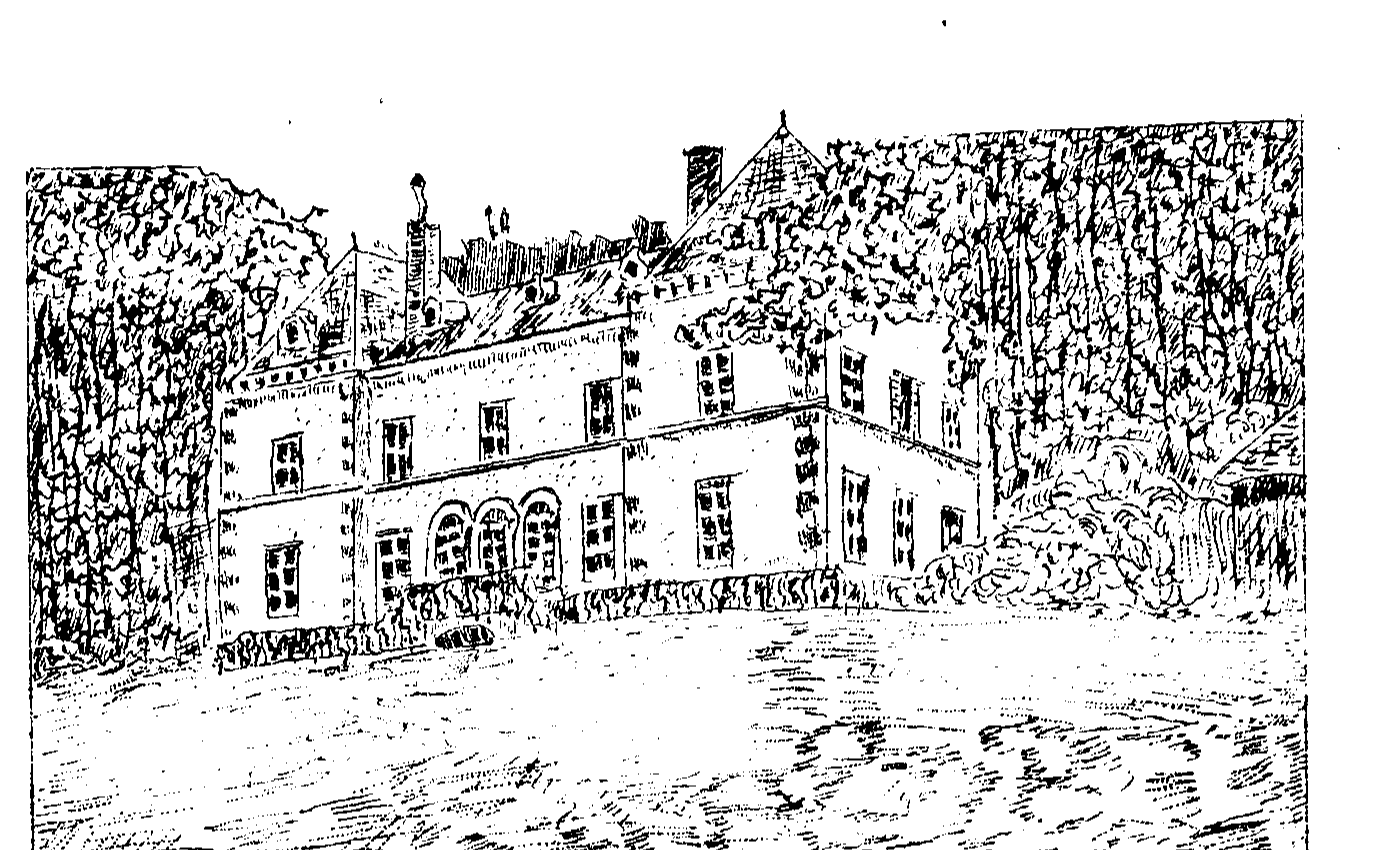
\includegraphics[width=0.72\textwidth]{Illustrations/illus-grosbois-chateau.png}
    \ourouxcaption{Château actuel construit en 1851}
\end{figure}

La terre de Gros-Bois fut érigée en fief en 1675 en faveur de Jean Chrysostôme de Grosbois, écuyer, seigneur de Rochetaillée, capitaine enseigne au régiment de Certirane.

Ses ancêtres portaient le nom de Massuyer et possédaient, dans la paroisse d'Ouroux, les domaines du Planet de Laye. Cette famille paraît s'être partagée en deux branches ; l'une se fixe à Tramayes, l'autre à Ouroux et à St-Mamert.

Voici du reste, les noms que nous avons pu recueillir dans les actes de cette époque.

Hugonin et Jean Massuyer, alias de Laye, figurent dans le terrier de Vauxrenard en 1459.

% --- Page imprimée 63 — vue 66
Le terrier d'Alloignet, de 1498, nous parle de Guyot Massuyer ; autrement du Planet, de Claude et Pierre Massuyer, autrement de Grosbois. Enfin celui de 1521 cite les frères de Grosbois, et François Massuyer de Tramayes qui possédait une terre au bourg d'Ouroux, "jouxt la maison Guillaume Bertet, près du pont sur la rivière de Grosne". Ce dernier prend même plus tard le nom de Grosbois, ce qui permettrait de supposer que la branche des Massuyer de Grosbois s'éteignit à la mort des frères Simon et Jean, laissant comme héritiers les Massuyer de Tramayes. Ce qui semblerait confirmer cette hypothèse, c'est que nous trouvons en 1660 Guillaume Massuyer bourgeois à Tramayes "baillant à grangeage à Claude Tribollet un domaine appelé de Grosboys situé à Ouroux".

Guillaume Massuyer serait donc le père de Jean Chrysostôme en faveur duquel le domaine de Grosbois fut érigé en fief. Celui qui, à cette époque, voulait s'élever au-dessus de sa condition, devait embrasser la carrière des armes. Nous verrons un membre de la famille Montel d'Ouroux entrer au service du roi, devenir capitaine comme Jean Chrysostôme et après avoir obtenu une modeste retraite faire construire à Saint-Mamert un château semblable à celui de Grosbois.

Jean Chrysostôme épousa Marie de la Roche, fille de Benoît de la Roche, seigneur de la Roche, de Poncié, et du Bief et de demoiselle Pierrette Prévost. La famille de la Roche ne possédait pas encore le fief de Lacarelle qui fut acheté plus tard par Joseph de la Roche, petit neveu de Benoît.

Jean Chrysostôme avait pour sœur Marie Anne de Grosbois qui avait épousé Roger de Palfenière seigneur de Saint-Julien.

À une époque que nous ne saurions préciser, Jean Chrysostôme avait acquis le fief du Razey situé sur les limites de St-Mamert et d'Ouroux. Ce fief avait appartenu à Noble Jacques de Sirvinge, comme nous le prouve son testament passé en 1629 en faveur de Anne de Sirvinge, sa fille et femme de Charles de Sevelinge bourgeois de Lyon.

"L'estat des revenus des gentilshommes" donne en l'année 1656 au sieur de Grosbois, un revenu de 500 livres et "le roolle des grand tailles" nous apprend qu'il possédait en 1674 deux fermiers, à la Combe d'Aissard et un appentionnaire.

% --- Page imprimée 64 — vue 67
Plus tard David de la Roche épousa sa cousine germaine, Anne de Grosbois, qui lui porta en dot le fief du même nom.

David de la Roche testa le 15 août 1718 et institua pour son héritier universel Claude François de la Roche, son fils.

Claude François de la Roche, chevalier, naquit à Villefranche le 25 juin 1710. D'abord conseiller du roi au bailliage de Beaujolais, il fut ensuite conseiller aux conseils de Monseigneur le duc d'Orléans. Il mourut le 1er mars 1748.

Antoine Isidore Marie de la Roche, son fils entra aux mousquetaires de la garde du roi en 1766. Il fit partie de l'Assemblée de la Noblesse du Beaujolais, réunie pour l'élection des députés aux états généraux du royaume, le 16 mars 1789, et fut l'un des otages qui s'offrirent pour Louis XVI et sa famille, en 1791.

Il avait épousé par contrat du 6 août 1772, demoiselle Françoise Thérèse de Ferrary de Romans, fille d'Étienne Lambert de Ferrary, comte de Romans, lieutenant du roi des provinces de Bresse, Bugey et Valromey, ancien capitaine au régiment de Lyonnais et de dame Marguerite Charrier.

Antoine Isidore Marie de la Roche mourut sans postérité. Avec lui s'éteignit la branche aînée de la famille de la Roche.

\begin{wrapfigure}{l}{0.46\textwidth}
    \vspace{-0.8\baselineskip}
    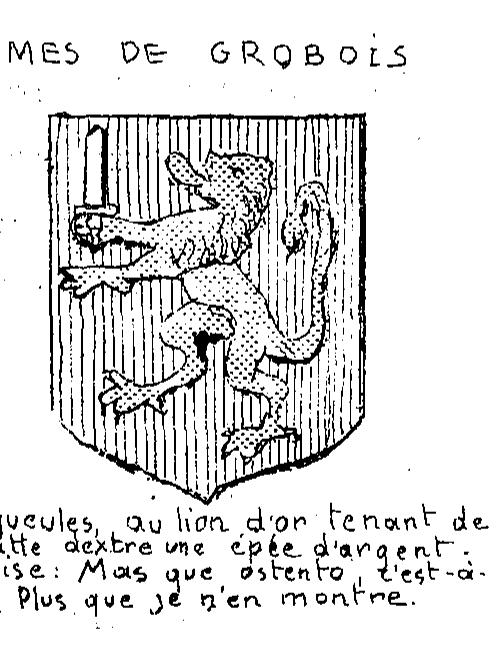
\includegraphics[width=0.43\textwidth]{Illustrations/illus-grosbois-armoiries.png}
\end{wrapfigure}

Grosbois appartient à la famille Berloty depuis 1842. François Félix Berloty, notaire à Lyon, avait acheté la plus grande partie du domaine et le château à MM. Solichon \& Pallaisson qui l'avaient acquis eux-mêmes un an auparavant de Monsieur de Lacarelle.

Cette propriété acquise en 1842 s'est augmentée petit à petit.
Monsieur Berloty, en 1852, fit démolir l'ancien château, vieille maison sans grand caractère et construisit à la même place l'habitation actuelle. Il traça le jardin et fit planter une partie de la forêt. Il fut maire d'Ouroux comme l'ont été après lui son fils et son petit-fils.

% --- Page imprimée 65 — vue 68
\begin{figure}[htbp]
    \centering
    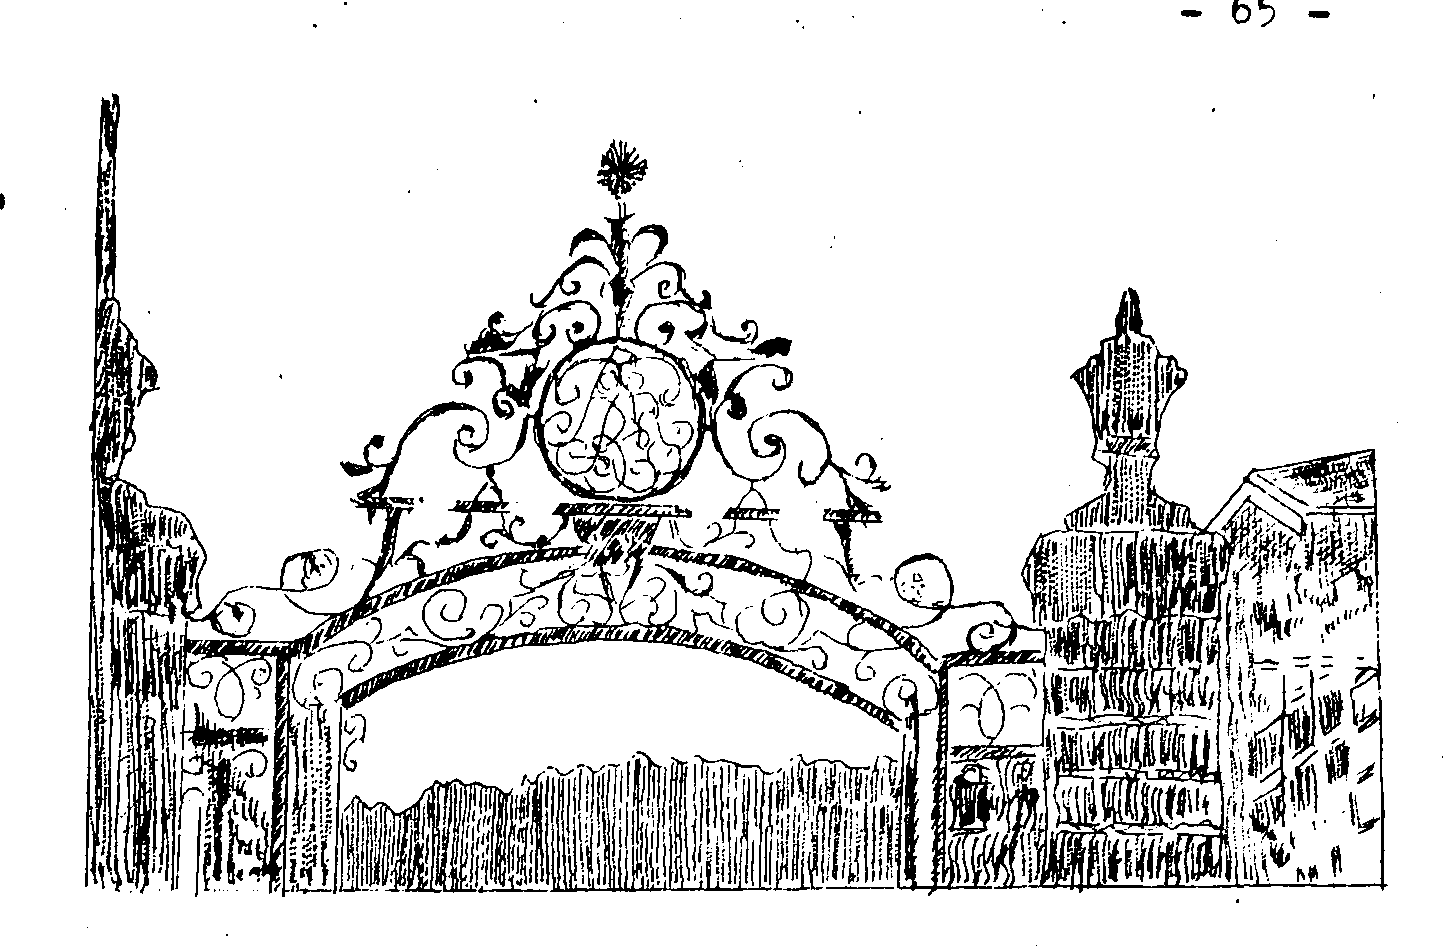
\includegraphics[width=0.72\textwidth]{Illustrations/illus-grosbois-imposte.png}
    \ourouxcaption{Belle imposte en fer forgé surmontant la porte d'entrée au château de GrosBois.}
\end{figure}

En terminant ce travail sur les fiefs de notre paroisse nous ne saurions passer sous silence une tradition d'après laquelle un château aurait existé près de Thel, au lieu appelé aujourd'hui Brousselaye ou broussailles de Laye. Cette tradition recueillie par Monsieur Morétain a été admise sans conteste par Ogier dans la France par Cantons. Devons-nous l'accepter à notre tour ? N'a-t-elle pas été surtout propagée par la lecture de cet ouvrage qui, à son apparition, était dans toutes les mains ? Passons sous silence la destruction du manoir, l'ensevelissement du châtelain sous ses ruines, l'existence de trésors découverts par la baguette divinatoire. Nous avons connu l'auteur du récit fait à Monsieur Morétain ; sa bonne foi a pu être facilement surprise.

Quant aux preuves historiques, elles font complètement défaut.

L'un et l'autre auteur prétend que le Roi fut mis en possession, le 5 Janvier 1749, de la Seigneurie de Laye d'Ouroux et de celle de Chamelet. Or, il s'agit ici non de Laye mais bien de Lay dans le Rhône.

D'autre part, dans la France par Cantons, à l'article St-Lager, nous lisons : "Par acte passé le lundi après Reminiscere de l'an 1339 Edouard de Beaujeu échangea avec noble et puissant seigneur Etienne de Laye tout ce qu'il possédait sur les communes de St-Lager et de

% --- Page imprimée 66 — vue 69
Cercié... contre les possessions qu'avait Étienne de Laye dans la paroisse d'Ouroux près de Villefranche". Or, ici encore, il ne s'agit pas d'Ouroux mais de Horons près Villeneuve en Dombes. On comprend que Monsieur Morétain ne pouvant vérifier l'exactitude de ces deux documents, ait admis la réalité de l'existence du château de Laye dans nos montagnes.

Ajoutons qu'on voit dans une ferme du Thel (ferme Ruet) un chapiteau roman historié, servant d'abreuvoir et provenant, dit-on, des ruines de ce château.

Devons-nous rejeter absolument la tradition ? Il est incontestable qu'autrefois quelques constructions s'élevaient sur le sommet de Brousselaye ; les amas de pierres et les débris de murailles en font foi. Mais la montagne elle-même ne figure jamais sous ce nom dans les terriers. Nous serions portés à croire que là se trouvait le Mas Chastard dont l'existence est attestée dans l'articulat Duligier et dont le souvenir a complètement disparu parmi nous. Du moins savons-nous qu'il était à peu de distance des Monnet et de Loifer dans cette vallée du Thel.

Quoiqu'il en soit aucun des titres anciens que nous avons pu consulter ne fait allusion à l'existence de ce château et aucune des preuves alléguées jusqu'à cette heure ne nous permet de donner une réponse affirmative.

\begin{figure}[htbp]
    \centering
    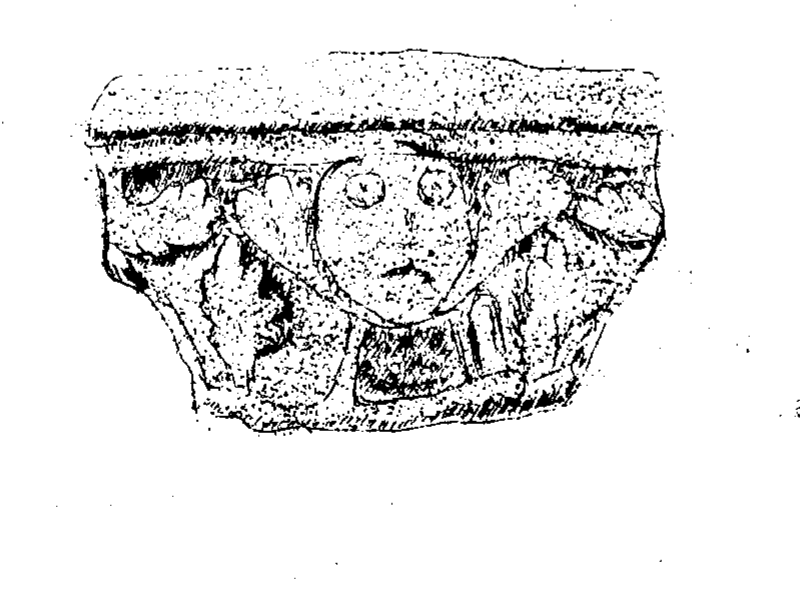
\includegraphics[width=0.42\textwidth]{Illustrations/illus-grosbois-chapiteau.png}
    \ourouxcaption{Chapiteau roman historié dans une ferme du Thel.}
\end{figure}
